\documentclass[10pt]{amsart}
% \usepackage[showboxes]{textpos}

\usepackage[absolute,overlay]{textpos}
	\setlength{\TPHorizModule}{1.0cm}
	\setlength{\TPVertModule}{\TPHorizModule}
	\textblockorigin{0.0cm}{0.0cm}  %start all at upper left corner

\usepackage{lmodern}
\usepackage{amsmath}
\usepackage{amsthm}
\usepackage{amsfonts}
\usepackage{amssymb}
\usepackage{mathpazo}
\usepackage{booktabs}
\usepackage[usenames,x11names]{xcolor}
\usepackage{tikz}
\usepackage{textcomp}
\usepackage[letterpaper]{geometry}
\geometry{verbose,tmargin=0.5in,bmargin=0.5in,lmargin=0.75in,rmargin=0.5in}
\usepackage{multicol}
\usepackage{bm}
\usepackage{comment}
\usepackage{cancel}
\usepackage{array}
\usepackage{gensymb}
\usepackage{enumerate}

\pagestyle{plain}
\raggedright
\renewcommand{\familydefault}{\sfdefault}
\setlength{\parskip}{\medskipamount}
\setlength{\columnsep}{1cm}

\everymath{\displaystyle}
\setlength{\parskip}{\bigskipamount}

\input{../../macros}

\begin{document}

\thispagestyle{empty}
\vspace{-7cm}
\centering

\textbf{\Large Module 7: Series A Pipeline (CIVL 318)}
\par\medskip


%%%%%%%%%%%%%%%%%%%%%%%%%%%%%%%%%%%%%%%%%%%%%%%%%%%%%%%%%%%%%%%%%%%%%%%%%%%%%%%%%%%%%%%%%%%%%%%%%%%%%%%%%%%%%%%%%%%%%

%\rule{\textwidth}{0.02in}
%%%%%%%%%%%%%%%%%%%%%%%%%%%%%%%%%%%%%%%%%%%%%%%%%%%%%%%%%%%%%%%%%%%%%%%%%%%%%%%%%%%%%%%%%%%%%%%%%%%%%%%%%%%%%%%%%%%%%
\raggedright




%%%%%%%%%%%%%%%%%%%%%%%%%%%%%%%%%%%%%%%%%%%%%%%%%%%%%%%%%%%%%%%%%%%%%%%%%%%%%%%%%%%%%%%%%%%%%%%%%%%%%%%%%
\mini[0.45]{




	\textbf{Example 1}:


	A pump delivers 13.5 L/s of kerosene at $25^\circ$C from an underground vented
	storage tank to an elevated storage tank pressurized to 745 kPa.
	\par
	The suction pipe is 6-in Schedule 40 steel pipe and is $5.0\,\text{m}$ long. It has a round-edged entrance with a radius
	of $r=15$ mm.
	\par
	The discharge pipe is 3-in Schedule 40 steel pipe,  is $11.0\,\text{m}$ long and includes a fully open butterfly valve
	with $L_e/D=45$.
	\par
	All elbows are ``standard'' with $L_e/D=30$.
	\parb
	\textbf{Solution}:
}
\hfill
\mini[0.5]{
	\cfig[0.4]{../../Figs/07SeriesPipeline/ElevStorA}
}





\vfill
\newpage
.
\newpage
.
\newpage







%%%%%%%%%%%%%%%%%%%%%%%%%%%%%%%%%%%%%%%%%%%%%%%%%%%%%%%%%%%%%%%%%%%%%%%%%%%%%%%%%%%%%%%%%%%%%%%%%%%%%%%%%


\textbf{Example 2}:

Gasoline at $25\text{ \textcelsius}$ flows under gravity from tank $A$ to tank $B$; both tanks are open to the
atmosphere.

The $2$-in Schedule $40$ steel pipe has a square entrance is $45.7\text{	m}$ long. The $4$-in Schedule $40$ steel
pipe contains a fully-open globe valve and is $87.5\text{ m}$ long. There is a sudden enlargement between the two
pipes, as shown. Both pipes are new commercial steel. All elbows are standard $90\degree$.

Determine the difference in surface elevation between tanks $A$
and $B$ required to maintain a flow of $425\text{ L/min}$.

\cfig[0.5]{../../Figs/07SeriesPipeline/07SeriesFindY}




\vfill
\newpage
.\newpage
.\newpage



%%%%%%%%%%%%%%%%%%%%%%%%%%%%%%%%%%%%%%%%%%%%%%%%%%%%%%%%%%%%%%%%%%%%%%%%%%%%%%%%%%%%%%%%%%%%%%%%%%%%%%%%%


\textbf{Example 3}:

Water at $25\text{ \textcelsius}$ is pumped from tank $A$ to tank $B$.
Both tanks are open to the atmosphere.

The suction pipe is $4\text{-in}$ Schedule $40$ steel pipe, has a well-rounded ($r/D>0.15$) entrance, contains a fully
open globe valve, and is $17.0\text{ m}$ long. The discharge pipe is $3\text{-in}$ Schedule $40$ steel pipe, contains a fully open globe valve and
three standard $90\degree$ elbows; it is $163.3\text{ m}$ long.

The elevation difference between $A$ and $B$ is $12.75\text{ m}$ and the volume flow rate is $Q=900\text{ L/min}$.

If the pump is $78\%$ efficient, determine the electrical power it uses.

\cfig[0.5]{../../Figs/07SeriesPipeline/07SeriesPump}


\vfill
\newpage
.\newpage
.\newpage

%%%%%%%%%%%%%%%%%%%%%%%%%%%%%%%%%%%%%%%%%%%%%%%%%%%%%%%%%%%%%%%%%%%%%%%%%%%%%%%%%%%%%%%%%%%%%%%%%%%%%%%%%

\textbf{Example 4}:

\mini[0.45]{
	Heavy machine oil (sg=$0.89$ and $\eta=3.80\times10^{-2}\mathsf{\ Pa\cdot s}$) is circulated through a system repeatedly to test its stability. \par\medskip
	The 8-inch Schedule steel pipe on the suction side of the pump has a square entrance and a length of $6.25$ m and the
	3.5-inch Schedule steel pipe on the discharge side of the pump has a length of $18.0$ m. All elbows are long
	radius. The flow rate through the system is $13.5$ L/s. \par\medskip
	Determine the head added by the pump.
}
\hfill
\mini[0.5]{
	\cfig[0.35]{../../Figs/07SeriesPipeline/07SeriesCycleOil}
}

\vfill

\newpage
.\newpage


%
% \textbf{Example 5}:
%
%
%
%
% The system illustrated is a pumped storage system. During periods of high demand for electricity, water flows down
% from the upper lake and drives the turbine at $D$. (During periods of low demand when electricity is cheap, such as at
% night-time, $D$ acts as a pump and pumps water back up to the upper lake.)
% \par\medskip
% At times of maximum demand, the system has a maximum volume flow rate of $420\;\mathsf{m^3/s}$. Base your
% calculations on this flow. The water is at $10\text{\textcelsius}$.
% \par\medskip
% The difference in elevation between the surfaces of the two lakes is $542\text{	m}$. \par\medskip
% The low pressure tunnel from $A$ to $B$ is $1700\text{ m}$ in length, has a diameter of $10.5\text{ m}$
% and is lined with concrete. The shaft and high pressure tunnel from $B$ to $D$ is $1140\text{ m}$ in length, has a diameter of $10.5\text{ m}$ and
% is lined with welded steel.
% \par\medskip
% There are three tailrace tunnels from the turbine to the lower reservoir with the flow equally
% distributed between them. Each tailrace tunnel is $382\text{ m}$ in
% length, has a diameter of $8.5\text{ m}$ and is lined with concrete.
%
% \par\medskip
% The entrance to the low pressure tunnel at the upper lake has an equivalent length ratio of $Le/D=420$. The bends at
% $B$ and $C$ are in the steel pipe and each have at equivalent length ratio of $16$. A spherical valve at the
% inlet of the turbine that shuts off flow when the turbines are not operating is hydraulically efficient and has no
% losses associated with it. Each tailrace tunnel contains a butterfly valve ($Le/D=20$).
% \par\medskip
% At maximum capacity, the turbine outputs $1800 \text{ MW}$. Determine the efficiency of the turbine at this output.
%
% \cfig[0.5]{../../Figs/07SeriesPipeline/series2}
% \textbf{Solution}:\\
%
% \vfill
% 	\newpage
% 	%%%%%%%%%%%%%%%%%%%%%%%%%%%%%%%%%%%%%%%%%%%%%%%%%%%%%%%%%%%%%%%%%%%%%%%%%%%%%%%%%%%%%%%%%%%%%%%%%%%%%%%%%%%%%%%%%%%%%
	\cmini{
		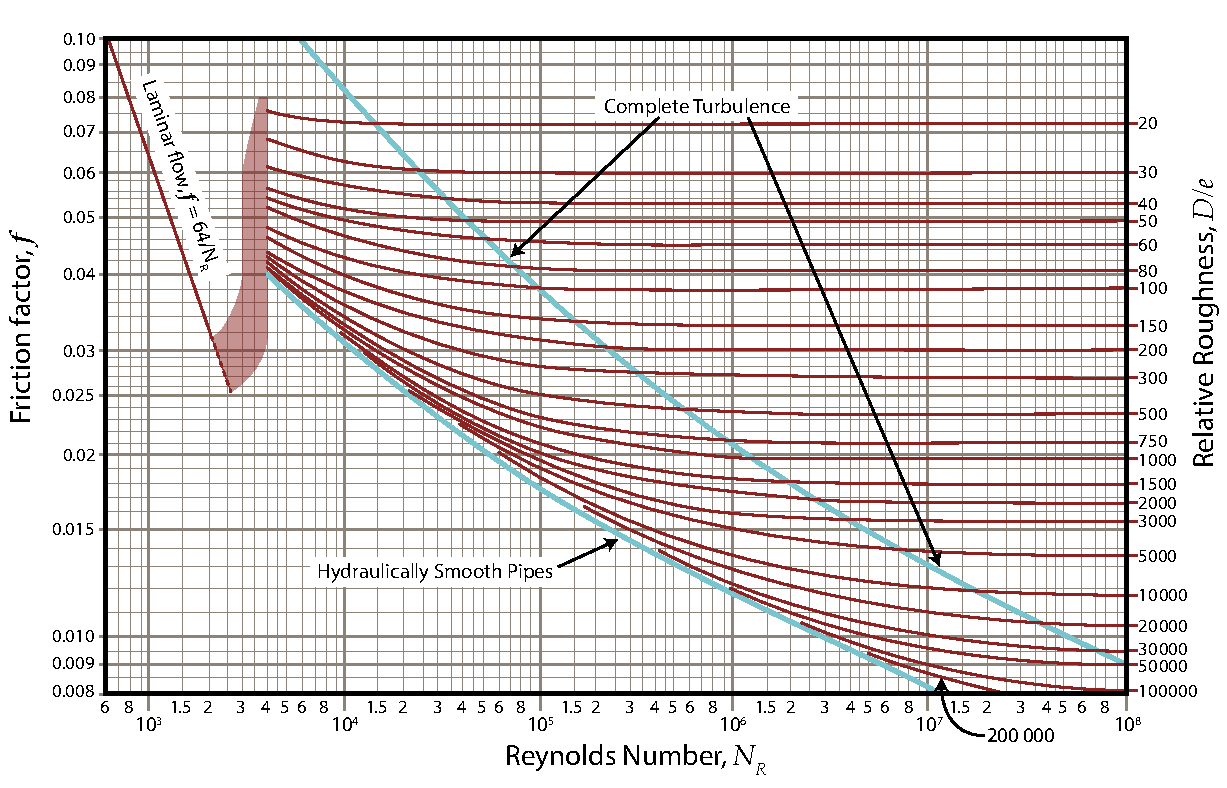
\includegraphics[angle=-90,scale=1.2]{../../Figs/07SeriesPipeline/moody}
	}



\end{document}
